\section{Group-Like Structures} 

\subsection{Semigroups and Monoids}

  Now the endowment of some structures gives rise to the following. Usually, we will start with the most general algebraic structures and then as we endow them with more structure, we can prove more properties. 

  \begin{definition}[Semigroup]
    A \textbf{semigroup} $(S, *)$ is a set $S$ with an associative binary operation. 
  \end{definition} 

  \begin{definition}[Monoid]
    A \textbf{monoid} $(M, *)$ is a semigroup with an identity element $1 \in M$ such that given a $m \in M$
    \begin{equation}
      1 * m = m * 1 = m
    \end{equation}
  \end{definition}

  Groupoids aren't necessarily that interesting, but there are cases in which semigroups and monoids come up. 

  \begin{example}[Continuous Time Markov Chain]
    Let $(\Omega, \mathcal{F}, \mathbb{P})$ be a probability space and $(S, \mathcal{S})$ a measurable space. Then, a homogeneous continuous-time Markov chain is a stochastic process $\{X_t\}_{t \geq 0}$ taking values in $S$ (i.e. $X_t: \Omega \rightarrow S$) satisfying the \textbf{Markov property}: for every bounded measurable $f$ and and $t, s \geq 0$, 
    \begin{equation}
      \mathbb{E}[ f(X_{t + s}) \mid \{X_r\}_{r \leq t} ] = \mathbb{E}[ f(X_{t + s}) \mid X_t ] = (P_s f)(X_t)
    \end{equation}
    The set $\{P_t\}_{t \geq 0}$ is called the \textbf{Markov semigroup}. 
  \end{example} 

  \begin{example}[Monoid of Transformations]
    Given a set $S$, consider the set of all functions $f: S \rightarrow S$. This forms a monoid with the identity function $f(x) = x$ as the identity element. Proof of associativity is shown in my set theory notes. 
  \end{example} 

  \begin{theorem}[Cardinality of Monoid of Transformations]
    If $|S| = n$, then the monoid of transformations has cardinality $n^n$. 
  \end{theorem}

  \begin{example}
    Let $S$ be any nonempty set. Then $(2^S, \cup, \emptyset)$ and $(2^S, \cap, S)$ are monoids. 
  \end{example}

  We first should ask whether the identity is unique in a monoid. It turns out it is. 

  \begin{lemma}[Uniqueness of Monoid Identity]
    The identity $1$ of a monoid $M$ is unique. 
  \end{lemma}
  \begin{proof}
    Assume not, i.e. there are 2 identities $1 \neq 1^\prime$. But then 
    \begin{equation}
      1 = 1 1^\prime = 1^\prime \implies 1 = 1^\prime
    \end{equation}
    where the implication follows from transitivity of equivalence relations. 
  \end{proof} 

  \begin{definition}[Submonoid]
    Given a monoid $(M, \ast)$, let $M^\prime \subset M$. If the restriction of $\ast$ to $M^\prime \times M^\prime$ is closed in $M^\prime$, then we can define the \textbf{submonoid} $(M^\prime, \ast)$. 
  \end{definition} 

  \begin{theorem}[Identities of Submonoids]
    If $M^\prime$ with identity $1^\prime$ is a submonoid of $M$ with identity $1$, Then $1 = 1^\prime$. 
  \end{theorem}
  \begin{proof}
    Assume not. $1^\prime \in M$, which means that 
  \end{proof}

\subsection{Groups}
  
  \begin{definition}[Group]
    A \textbf{group} $(G, \ast)$ is a set with binary operation $x \ast y$---also written as $xy$---having the following properties.\footnote{Note that this is a monoid with the additional property of inverses.}
    \begin{enumerate}
      \item \textit{Closure}. $x, y \in G \implies xy \in G$\footnote{but not necessarily $xy  = yx$}
      \item \textit{Associativity}. $\forall x, y, z \in G, x(yz) = (xy)z$
      \item \textit{Identity}. $\exists e \in G$ s.t. $\forall x \in G, xe = ex = x$
      \item \textit{Inverses}. $\forall x \in G \; \exists x^{-1} \in G$ s.t. $x x^{-1} = x^{-1} x = e$
    \end{enumerate}
    The \textbf{order} of a group is the cardinality $|G|$. 
  \end{definition} 

  This is an extremely simple structure, and the first thing we should prove is the uniqueness of the identity and inverses. 

  \begin{lemma}[Uniqueness of Identity and Inverse]
    The identity and the inverse is unique, and for any $a, b$, the equation $x*a = b$ has the unique solution $x = b* a^{-1}$.
  \end{lemma}
  \begin{proof}
     Assume that there are two identities of group $(G,*)$, denoted $e_{1}, e_{2}$, where $e_{1} \neq e_{2}$. According to the properties of identities, $e_{1} = e_{1} * e_{2} = e_{2} \implies e_{1} = e_{2}$. \\
    As for uniqueness of a inverses, let $a$ be an element of $G$, with its inverses $a_{1}^{-1}, a_{2}^{-1}$. Then, 
    \begin{align*}
      a * a_{1}^{-1} = e & \implies a_{2}^{-1} * \Big(a * a_{1}^{-1} \Big)= a_{2}^{-1} * e \\
       & \implies \Big(a_{2}^{-1} * a \Big) * a_{1}^{-1} = a_{2}^{-1} \\
       & \implies e * a_{1}^{-1} = a_{2}^{-1}
    \end{align*}
    Since the inverse is unique, we can operate on each side of the equation $x*a = b$ to get $x*a*a^{-1} = b*a^{1} \implies x * e = x = b*a^{-1}$. Clearly, the derivation of this solution is unique since the elements that we have operated on are unique.
  \end{proof} 
  
  At this point, we can see that for each group there is a corresponding ``multiplication table'' defined by the operation. For example, we can create a set of $6$ elements $\{r_0, r_1, r_2, s_0, s_1, s_2\}$ and define the operation $\times$ as the following. 

  \begin{figure}[H]
    \centering 
    \begin{tabular}{c|cccccc}
      $\times$ & $r_0$ & $r_1$ & $r_2$ & $s_0$ & $s_1$ & $s_2$ \\
      \hline
      $r_0$ & $r_0$ & $r_1$ & $r_2$ & $s_0$ & $s_1$ & $s_2$ \\
      $r_1$ & $r_1$ & $r_2$ & $r_0$ & $s_1$ & $s_2$ & $s_0$ \\
      $r_2$ & $r_2$ & $r_0$ & $r_1$ & $s_2$ & $s_0$ & $s_1$ \\
      $s_0$ & $s_0$ & $s_2$ & $s_1$ & $r_0$ & $r_2$ & $r_1$ \\
      $s_1$ & $s_1$ & $s_0$ & $s_2$ & $r_1$ & $r_0$ & $r_2$ \\
      $s_2$ & $s_2$ & $s_1$ & $s_0$ & $r_2$ & $r_1$ & $r_0$ \\
    \end{tabular}
    \caption{Multiplication table for some random (or is it?) group. Note that we can only write such a table explicitly for a group of finite elements. But even for arbitrary groups, we should think of the operation completely defining a possibly ``infinite'' table.} 
  \end{figure} 

  \begin{example}[Group of Invertible Elements of a Monoid]
    
  \end{example}

  Let's prove a little more about groups so that we have more tools for manipulation. 

  \begin{lemma}[Properties of Group Operation]
    Given $a, b, c \in G$, 
    \begin{enumerate}
      \item $ab = cb \implies a = c$. 
      \item $\forall a \in G$, $(a^{-1})^{-1} = a$. 
      \item $(ab)^{-1} = b^{-1} a^{-1}$. 
    \end{enumerate}
  \end{lemma}
  \begin{proof}
    TBD. 
  \end{proof}

  \begin{definition}[Subgroup]
    Given group $(G, \ast)$ and $(G^\prime, \ast)$ with the same operations, $G^\prime$ is a \textbf{subgroup} of $G$ if $G^\prime \subset G$. 
  \end{definition} 

  \begin{definition}[Abelian Group]
    An \textbf{abelian group} $(A, +)$ is a group where $+$ is commutative.\footnote{Note that I switched the notation from $\ast$ to $+$. By convention and to avoid confusion, $+$ denotes commutative operations. }
  \end{definition} 

  It is clear that in an abelian group, the multiplication table must be symmetric across the diagonal. 

  \begin{example}[Abelian Groups]
    Here are some examples. 
    \begin{enumerate}
      \item $\mathbb{Z}, \mathbb{Q}, \mathbb{R}$ are all abelian groups with respect to addition. $\mathbb{Q}^{*} \equiv \mathbb{Q} \setminus \{0\}$ and $\mathbb{R}^{*} \equiv \mathbb{R} \setminus \{0\}$ are abelian groups with respect to multiplication.
      \item The set of all functions on a given interval $[a,b]$ is abelian with respect to addition, defined as $(f+g)(x) \equiv f(x) + g(x)$. 
    \end{enumerate}
  \end{example} 

\subsection{Group Homomorphisms}

  At this point, we would like to try and classify groups (e.g. can we find \textit{all} possible groups of a finite set?). But consider the two groups. 

  \begin{figure}[H]
    \centering
    \begin{subfigure}[b]{0.48\textwidth}
      \centering
      \begin{tabular}{c|ccc}
        \hline
        $+$ & 0 & 1 & 2 \\
        \hline
        0 & 0 & 1 & 2 \\
        1 & 1 & 2 & 0 \\
        2 & 2 & 0 & 1 \\
        \hline
      \end{tabular}
    \end{subfigure}
    \hfill 
    \begin{subfigure}[b]{0.48\textwidth}
      \centering
      \begin{tabular}{c|ccc}
        \hline
        $+$ & a & b & c \\
        \hline
        a & a & b & c \\
        b & b & c & a \\
        c & c & a & b \\
        \hline
      \end{tabular}
    \end{subfigure}
    \caption{Two isomorphic groups.}
  \end{figure} 

  These groups have different elements, but the operation behaves in exactly the same way between them (it may be a little harder if I relabeled the elements or permuted the rows/columns). Since we can trivially make arbitrary sets there really isn't much meaning to having two versions of the same group (at least in the algebraic sense). Therefore, these groups should be labeled ``equivalent'' in some way, and we will precisely define this notion now. 

  \begin{definition}[Group Homomorphism]
    Let $(G, \circ)$ and $(H, *)$ be two groups. The mapping $f: (G, \circ) \longrightarrow (H, *)$ is a \textbf{group homomorphism} if for all $a, b \in G$, 
    \begin{equation}
      f(a \circ b) = f(a) * f(b)
    \end{equation} 
    Furthermore, 
    \begin{enumerate}
      \item A \textbf{group isomorphism} is a bijective group homomorphism, and we call groups $M, N$ \textbf{isomorphic}, denoted $M \simeq N$, if there exists an isomorphism between them. 
      \item An \textbf{endomorphism} is a homomorphism from a group to itself. 
      \item An \textbf{automorphism} is a isomorphism from a group to itself. 
    \end{enumerate}
  \end{definition} 

  It turns out that from the simple property that $f(ab) = f(a) f(b)$, it also maps identities to identities, and inverses to inverses!  

  \begin{lemma}[Homomorphisms Maps Identities/Inverses to Identities/Inverses]
    Given a homomorphism $f: (G, \ast) \rightarrow (H, \times)$ and $a \in G$, 
    \begin{equation}
      f(e_G) = e_H, \qquad f(a^{-1}) = f(a)^{-1}
    \end{equation}
  \end{lemma}
  \begin{proof}
    Let $a \in G$. Then 
    \begin{equation}
      f(a) = f(a e_G) = f(a) f(e_G) \implies e_H = f(a)^{-1} f(a) = f(a)^{-1} f(a) f(e_G) = f(e_G)
    \end{equation}
    To prove inverses, we see that 
    \begin{equation}
      f(a) f(a^{-1}) = f(a a^{-1}) = f(e_G) = e_H
    \end{equation}
    from above, and this implies that $f(a^{-1}) = f(a)^{-1}$. We can also do this with right hand side multiplication. 
  \end{proof}

  \begin{example}[Exponential Map]
    The map $a \mapsto 2^{a}$ is an isomorphism between $(\mathbb{R}, +)$ and $(\mathbb{R}^{+}, \times)$ since 
    \begin{equation}
      2^{a+b} = 2^a \times 2^b
    \end{equation} 
    which is proved in my real analysis notes when constructing the exponential map on the reals. 
  \end{example} 

  \begin{example}[Determinant]
    The determinant $\det: \GL_n (\mathbb{F}) \rightarrow \mathbb{F}^\ast$ is a homomorphism because of the product rule for determinants. 
  \end{example}

  Therefore, we can see that an isomorphism is really just a ``renaming'' of the elements, which aligns with our view of equivalence as above. Not only does it renamee the elements, but it preserves all the algebraic properties of the group and each element. 

  \begin{theorem}[Preservation of Properties in Isomorphism]
    If $f: G \rightarrow H$ is an isomorphism, then 
    \begin{enumerate}
      \item $f^{-1}$ is also an isomorphism. 
      \item $|G| = |H|$.
      \item $\forall a \in G$, $\ord(a) = \ord(f(a))$. 
      \item $G$ is abelian $\implies H$ is abelian. 
    \end{enumerate} 
  \end{theorem}
  \begin{proof}
    Listed. 
    \begin{enumerate}
      \item Since $f$ is bijective by definition, $f^{-1}$ is well-defined and bijective as well. Now we show that $f^{-1}$ is a group homomorphism. Given $c, d \in H$, take 
      \begin{equation}
        f \big( f^{-1} (c), f^{-1} (d)\big) = f \big( f^{-1} (c) \big) \, f \big( f^{-1} (d) \big) = cd 
      \end{equation}
      where the first equality follows since $f$ is a homomorphism, and the second since $f^{-1}$ is the inverse mapping. Now mapping both sides through $f^{-1}$, we get 
      \begin{equation}
        f^{-1} (c) f^{-1} (d) = f^{-1} (cd)
      \end{equation}
      and so $f^{-1}$ is a homomorphism. 

      \item This is trivial by bijectivity. 
      \item TBD. 
      \item Let $c, d \in H$. Then $c = f(a), d = f(b)$ for some $a, b \in G$, and so $cd = f(a) f(b) = f(ba) = f(b) f(a) = dc$. 
    \end{enumerate}
  \end{proof}

  A trivial example is the identity map, which is an automorphism. But can we generalize this a bit better? 

  \begin{theorem}
    Let $G$ be a group with $a \in G$. Then the following is an automorphism on $G$. 
    \begin{equation}
      \phi: G \longrightarrow G, \; \phi (x) = a x a^{-1}
    \end{equation}
  \end{theorem}
  \begin{proof}
    The map $\psi: G \longrightarrow G, \; \psi(x) = a^{-1} x a$ is clearly the inverse of $\phi$, with $\phi \psi = \psi \phi = I$ for all $x \in G \implies \phi$ is bijective. Secondly, $\phi(x) \phi(y) = a x a^{-1} a y a^{-1} = a (x y) a ^{-1} = \phi (x y) \implies \phi$ preserves the group structure. 
  \end{proof} 

  \begin{definition}[Kernel]
    Given group homomorphism $f: G \rightarrow H$, the \textbf{kernel} of $f$ is defined 
    \begin{equation}
      \ker(f) \coloneqq \{g \in G \mid f(g) = e_H\}
    \end{equation}
    That is, it is the preimage of the identity. 
  \end{definition} 

  \begin{theorem}[Kernels are Subgroup]
    Given a group homomorphism $f: G \rightarrow H$, 
    \begin{enumerate}
      \item $\ker(f)$ is a subgroup of $G$.  
      \item $f$ is injective $\iff \ker(f) = \{e_G\}$. 
    \end{enumerate}
  \end{theorem}
  \begin{proof}
    For the first part, we prove the properties of a group. To show closed, consider $a, b \in \ker(f)$. Then $f(ab) = f(a) f(b) = e_H e_H = e_H \implies ab \in \ker(f)$. Since $f(e_G) = e_H$, $e_G \in \ker(f)$. If $a \in \ker(f)$, then $f(a^{-1}) = f(a)^{-1} = e_H^{-1} = e_H \implies a^{-1} \in \ker(f)$. Finally associativity follows from associativity of the supgroup. 

    For the second part, we prove bidirectionally. 
    \begin{enumerate}
      \item $(\rightarrow)$. Since $f$ is injective, $f(a) = f(b) \implies a = b$. Let $a \in \ker(f)$. Then $f(a) = e_H$, and so $f(e_G) = e_H = f(a)$. By injectivity, $a = e_G$, and so $\ker(f) = \{e_G\}$. 
      \item $(\leftarrow)$. Let $a, b \in G$ s.t. $f(a) = f(b)$. Then $f(a) f(b)^{-1} = e_H \implies af(a) f(b^{-1}) = f(a b^{-1}) = e_H \implies ab^{-1} \in \ker(f)$. But by hypothesis $\ker(f) = \{e_G\} \implies ab^{-1} = e_G \implies a = b$. 
    \end{enumerate}
  \end{proof}

  \begin{example}[Projection onto Unit Circle]
    Given $\mathbb{C}^\ast = \mathbb{C} \setminus \{0\}$ with $\times$ and $S^1 = \{x \in \mathbb{C} \mid |x| = 1\}$ (which is a group under multiplication), the map $f: \mathbb{C}^\ast \rightarrow S^1$ defined $f(z) = z/|z|$ is a group homomorphism since 
    \begin{equation}
      f(z_1 z_2) = \frac{z_1 z_2}{|z_1 z_2|} = \frac{z_1 z_2}{|z_1| |z_2|} = f(z_1) f(z_2)
    \end{equation}
  \end{example} 

\subsection{Group Presentations} 

  A group $G$ may be very abstract and complicated, and so working with all its elements can be a bit painful. It would be more useful to work with a smaller subset $S$ of $G$ that can completely characterize $G$.\footnote{Note that this is similar to the basis that generates a topology.} We would like to formalize this notion, which will be very useful later on. For now, let's start off with a simple element $a \in G$, and perhaps we can consider the elements 
  \begin{equation}
    \ldots, a^{-2}, a^{-1}, a^0 = e, a^1, a^2, \ldots
  \end{equation}
  It may or may not be the case that $a$ may cycle back to itself for some $n$, i.e. $a = a^n$. 

  \begin{definition}[Order of an Element]
    The \textbf{order} of a group element $a \in G$ is the minimum number $n \in \mathbb{N}$ s.t. $a = a^n$, denoted $|a|$ or $\ord(a)$.\footnote{Note that this is different from the order of a group. This is confusing, I know. }
  \end{definition} 

  Now the set of all multiples of $a$ may or may not be the group, but if we take a certain subset of these elements and take all multiples of all combinations of them, we may have better coverage of the group. 

  \begin{definition}[Word]
    A \textbf{word} is any written product of group elements and inverses. They are generally in the form
    \begin{equation}
      s_{1}^{\epsilon_{1}} s_{2}^{\epsilon_{2}} s_{3}^{\epsilon_{3}}... s_{k}^{\epsilon_{k}}, \text{ where} e_i \in \mathbb{Z}
    \end{equation} 
    e.g. given a set $\{x,y,z\}$, $x y, x z^{-1} y y x^{-2},...$ are words. 
  \end{definition}

  \begin{definition}[Generating Set]
    The \textbf{generating set} $\langle S \rangle$ of a group $G$ is a subset of $G$ such that every element of the group can be expressed as a word of finitely many elements under the group operations. The elements of the generating set are called \textbf{generators}.
  \end{definition}

  \begin{definition}[Free Group]
    The \textbf{free group} $F_{S}$ over a given set $S$ consists of all words that can be built from elements of $S$. 
  \end{definition}

  Now for notational convenience, one method of specifying a group is to put it in the form
  \begin{equation}
    \big\langle \; S \; | \; R \;\big\rangle
  \end{equation}
  where $S$ is the generating set and $R$ is a set of relations. This is called the \textit{group presentation}. 

  \begin{example}[Group Presentations]
    The cyclic group of order $n$ could be presented as
    \begin{equation}
      \big\langle \; a \; | \; a^{n} = 1 \;\big\rangle
    \end{equation}
    Dih $(8)$, with $r$ representing a rotation by $45$ degrees in the direction of the orientation and $f$ representing a flip over any axis, is presented by
    \begin{equation}
      \big\langle \; \{ r, f\} \; | \; r^{8} = 1, f^{2} = 1, (r f)^{2} = 1 \;\big\rangle
    \end{equation}
  \end{example}

  A lot of groups fall into one or more categories depending on what properties they have. We will proceed to just define these categories and introduce the groups as needed. 


  \begin{theorem}[Tip]
    To prove a group homomorphism, show that every element of $G$ and $H$ can be written as a word of certain $g_i$'s in $G$ and then $h_i$'s in $H$, and map the $g_i$'s to $h_i$'s. 
  \end{theorem}

  \begin{definition}[Cyclic Group]
    A \textbf{cyclic group}, denoted $Z_{n}$, is a group generated by a single element. In a \textbf{finite cyclic group}, there exists a $k \in \mathbb{N}$ such that $g^{k} = g^{0} = 1$ (or in additive notation, $kg = 0g = 0$), where $g$ is the generator. A \textbf{finitely generated group} is a group generated by a finite number of elements. In \textbf{infinite cyclic groups}, all elements are distinct for distinct $k$. 
  \end{definition} 

  \begin{example}[Cyclic Groups] 
    Here are some examples of cyclic groups. 
    \begin{enumerate}
      \item $(\mathbb{Z}_n, +)$, the integers mod $n$, is a cyclic group of order $n$, generated by $1$.\footnote{In fact, the generator of $\mathbb{Z}_n$ can be any integer relatively prime to $n$ and less than $n$.} 
      \item The $n$th roots of unity in $\mathbb{C}$ is a cyclic group of order $n$, generated by the counterclockwise rotation $e^{2\pi/n}$. 
      \item The set of discrete angular rotations in $SO(2)$, in the form of 
      \begin{equation}
        R =  \bigg\{ \begin{pmatrix}
        \sin{\theta} & \cos{\theta} \\
        \cos{\theta} & -\sin{\theta}
        \end{pmatrix}\; \bigg| \; \theta \in \Big\{\frac{2 \pi}{n} k\Big\}_{k = 0}^{n-1} \bigg\}
      \end{equation}

      \item $(\mathbb{Z}, +)$ is an infinite cyclic group. 
    \end{enumerate}
  \end{example}

  That's really it for cyclic groups, and to make things simpler, there is a complete characterization of them. 

  \begin{theorem}[Cyclic Groups are Unique up to Order]
    Given a cyclic group, $Z$ or $Z_n$ 
    \begin{enumerate}
      \item If it is finite, then $(Z_n, +) \simeq (\mathbb{Z}_n, +) \simeq \langle 1 \rangle$. 
      \item If it is infinite, then $(Z, +) \simeq (\mathbb{Z}, +) \simeq \langle 1 \rangle$. 
    \end{enumerate}
  \end{theorem}
  \begin{proof}
    
  \end{proof}

  Therefore, we have completely characterized all cyclic groups! However, note that there can be isomorphisms from a cyclic group to a subgroup. 

  \begin{example}[Integers to Even Integers]
    Let $2 \mathbb{Z}$ denote the set of all even integers with addition. Then we can verify that this is a group, and 
    \begin{equation}
      \mathbb{Z} \simeq 2 \mathbb{Z}
    \end{equation}
  \end{example}

  \begin{definition}[Polytope]
    A \textbf{polytope} in $n$-dimensions is a geometrical object with "flat sides, " called an n-polytope. It is a generalization of a polygon or a polyhedron to an arbitrary number of dimensions. 
  \end{definition}

  \begin{definition}[Simplex]
    A \textbf{n-simplex} is a n-polytope which is the n-dimensional convex hull of its $n+1$ vertices. Moreover, the $n+1$ vertices must be \textbf{affinely independent}, meaning that
    \begin{equation}
      \{u_1 - u_0, u_2 - u_0, ..., u_n - u_0 | \{u_i\}_{i=0}^{n} \text{ vertices} \}
    \end{equation}
    are linearly independent vectors that span the n-dimensional space. 
  \end{definition}

  \begin{definition}[Symmetry Group]
    The \textbf{symmmetry group} of a geometrical object is the group of all transformations in which the object is invariant. Preserving all the relevant structure of the object. 
  \end{definition}

  \begin{definition}[Dihedral Group]
    A common example of such groups is the \textbf{dihedral group} of order $2n$, with the group presentation 
    \begin{equation}
      \Dih(n) \coloneqq \langle r, f \mid r^n = f^2 = e, rfr = f  \rangle
    \end{equation}
    , denoted $\Dih(n)$ of order $2n$, which is the group of symmetries of a n-simplex, which includes rotations and reflections. 
  \end{definition}

  \begin{example}[$\Dih(3)$ on Triangle]
    The group of rotations and flips you can do on a equilateral triangle is called the Dihedral Group $\Dih(3)$. It is not abelian. 

    \begin{figure}[H]
      \centering 
      \begin{tabular}{|c|c|c|c|c|c|c|}
        \hline
        & $r_0$ & $r_1$ & $r_2$ & $s_0$ & $s_1$ & $s_2$ \\
        \hline
        $r_0$ & $r_0$ & $r_1$ & $r_2$ & $s_0$ & $s_1$ & $s_2$ \\
        \hline
        $r_1$ & $r_1$ & $r_2$ & $r_0$ & $s_1$ & $s_2$ & $s_0$ \\
        \hline
        $r_2$ & $r_2$ & $r_0$ & $r_1$ & $s_2$ & $s_0$ & $s_1$ \\
        \hline
        $s_0$ & $s_0$ & $s_2$ & $s_1$ & $r_0$ & $r_2$ & $r_1$ \\
        \hline
        $s_1$ & $s_1$ & $s_0$ & $s_2$ & $r_1$ & $r_0$ & $r_2$ \\
        \hline
        $s_2$ & $s_2$ & $s_1$ & $s_0$ & $r_2$ & $r_1$ & $r_0$ \\
        \hline
      \end{tabular}
      \caption{Multiplication table for $D_3$. } 
      \label{fig:triangle_d3}
    \end{figure}
  \end{example} 

  \begin{example}[Groups of Order 3]
    $\Dih(3) \simeq S_{3}$, since permutations of the vertices of a triangle are isomorphic to a permutations of a 3-element set. 
  \end{example}  

  However, $S_4$ is not isomorphic to the symmetry group of a square. It is however, isomorphic to that of a tetrahedron, i.e. $\Dih(4)$. 

  \begin{example}[Low Order Dihedral Group]
    We introduce some low order Dihedral groups. 
    \begin{enumerate}
      \item Dih$(3)$ is the group of all rotations and reflections that preserve the structure of the equilateral triangle in $\mathbb{R}^2$, a regular 2-simplex. 
      \begin{center}
      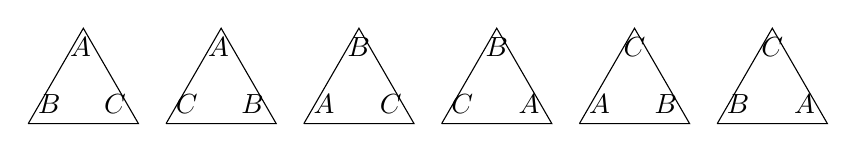
\begin{tikzpicture}[scale=0.7]
          \draw (-1,0)--(1,0)--(0,1.732)--(-1,0);
          \draw (-3.5,0)--(-1.5,0)--(-2.5,1.732)--(-3.5,0);
          \draw (-6,0)--(-4,0)--(-5,1.732)--(-6,0);
          \draw (4,0)--(6,0)--(5,1.732)--(4,0);
          \draw (1.5,0)--(3.5,0)--(2.5,1.732)--(1.5,0);
          \draw (6.5,0)--(8.5,0)--(7.5,1.732)--(6.5,0);
          \node[below] at (-5.05, 1.732) {$A$};
          \node[below] at (-2.55, 1.732) {$A$};
          \node[below] at (-0, 1.732) {$B$};
          \node[below] at (2.5, 1.732) {$B$};
          \node[below] at (5, 1.732) {$C$};
          \node[below] at (7.5, 1.732) {$C$};
          \node[above right] at (-6,0) {$B$};
          \node[above right] at (-3.5,0) {$C$};
          \node[above right] at (-1,0) {$A$};
          \node[above right] at (1.5,0) {$C$};
          \node[above right] at (4,0) {$A$};
          \node[above right] at (6.5,0) {$B$};
          \node[above left] at (-4.05,0) {$C$};
          \node[above left] at (-1.55,0) {$B$};
          \node[above left] at (0.95,0) {$C$};
          \node[above left] at (3.45,0) {$A$};
          \node[above left] at (5.95,0) {$B$};
          \node[above left] at (8.45,0) {$A$};
      \end{tikzpicture}
      \end{center}
      \item Dih$(4)$ is the group of all rotations and reflections that preserve the structure of the regular tetrahedron in $\mathbb{R}^{3}$. An incorrect, yet somewhat useful, way of visualizing this group is to imagine a square in $\mathbb{R}^{2}$. However, the points are not pairwise equidistant and therefore does not preserve symmetry between all points.
      \item Dih$(n)$ is similarly the group of all rotations and reflections that preserve the structure of a regular $(n-1)$-simplex in $\mathbb{R}^{n-1}$. 
    \end{enumerate}
  \end{example} 

  \begin{example}[Klein 4 Group]
    The \textbf{Klein 4-Group} can be described as the symmetry group of a non-square rectangle. With the three non-identity elements being horizontal reflection, vertical reflection, and 180-degree rotation. 

    \begin{figure}[H]
      \centering 
      \begin{tabular}{c|cccc}
        \hline
        $\cdot$ & $e$ & $a$ & $b$ & $c$ \\
        \hline
        $e$ & $e$ & $a$ & $b$ & $c$ \\
        $a$ & $a$ & $e$ & $c$ & $b$ \\
        $b$ & $b$ & $c$ & $e$ & $a$ \\
        $c$ & $c$ & $b$ & $a$ & $e$ \\
        \hline
      \end{tabular}
      \caption{Multiplication table for the Klein 4-group ($V_4$)} 
      \label{fig:klein4group}
    \end{figure}
  \end{example}

  \begin{example}[Groups of Order 4]
    There are only 2 groups of order 4. 
    \begin{figure}[H]
      \centering
      \begin{subfigure}[b]{0.48\textwidth}
        \centering
        \begin{tabular}{|c|c|c|c|c|}
          \hline
          $C_4$ & $e$ & $a$ & $a^2$ & $a^3$ \\
          \hline
          $e$ & $e$ & $a$ & $a^2$ & $a^3$ \\
          \hline
          $a$ & $a$ & $a^2$ & $a^3$ & $e$ \\
          \hline
          $a^2$ & $a^2$ & $a^3$ & $e$ & $a$ \\
          \hline
          $a^3$ & $a^3$ & $e$ & $a$ & $a^2$ \\
          \hline
        \end{tabular}
        \caption{Cyclic group $C_4$}
      \end{subfigure}
      \hfill 
      \begin{subfigure}[b]{0.48\textwidth}
        \centering
        \begin{tabular}{|c|c|c|c|c|}
          \hline
          $V$ & $e$ & $a$ & $b$ & $c$ \\
          \hline
          $e$ & $e$ & $a$ & $b$ & $c$ \\
          \hline
          $a$ & $a$ & $e$ & $c$ & $b$ \\
          \hline
          $b$ & $b$ & $c$ & $e$ & $a$ \\
          \hline
          $c$ & $c$ & $b$ & $a$ & $e$ \\
          \hline
        \end{tabular}
        \caption{Klein four-group $V$}
      \end{subfigure}
      \caption{Cayley tables for the two groups of order 4}
      \label{fig:order4groups}
    \end{figure} 
  \end{example}

\subsection{Symmetric and Alternating Groups}

  Notice that given any set $S$, we can define the set of all functions $f: S \rightarrow S$ as a monoid. What if we consider the set of all invertible functions? This by definition means bijective functions, and so consider this subset.  

  \begin{definition}[Symmetric/Transformation Group]
    Given a set $S$, the \textbf{transformation group}, or \textbf{symmetric group}, of $S$ is the group of all bijective maps from $S$ to itself. 
  \end{definition} 

  This exists for all sets $S$, and if $S$ is finite, we call it a \textbf{permutation group}, since the set of bijective transformations of it is a permutation of its elements. 

  \begin{definition}[Permutation Group]
    The \textbf{permutation group} is the set of all bijective transformations from any set $X$ to the same set, denoted either Sym$(X)$ or $S_n$. If $X = \{1, 2, 3 ,... , n\}$, known as the set of all permutations of $X$, with cardinality $n!$. 
  \end{definition}

  \begin{lemma}
    Every element in finite $S_{n}$ can be decomposed into a partition of cyclic rotations.
  \end{lemma}

  \begin{example}
    Listed.
    \begin{enumerate}
      \item $(1 2)$ is a mapping $1 \rightarrow 2,\; 2 \rightarrow 1$. 
      \item $(1 2 3)$ is a mapping $1\rightarrow 2,\; 2 \rightarrow 3,\; 3 \rightarrow 1$. 
      \item $(1 2 3) (4 5)$ is a mapping $1\rightarrow 2,\; 2 \rightarrow 3,\; 3 \rightarrow 1, \;4 \rightarrow 5, \;5 \rightarrow 4$. 
    \end{enumerate}
  \end{example}

  \begin{definition}
    The \textbf{conjugacy class} of $S_{n}$ correspond to the cycle structures of $S_{n}$. Two elements of $S_{n}$ are conjugate in $S_{n}$ if and only if they consist of the same number of disjoint cycles of the same lengths. 
  \end{definition} 

  \begin{example}
    \begin{enumerate}
      \item $(1 2 3) (4 5)$ is conjugate to $(1 4 3) (2 5)$.
      \item $(1 2) (4 5)$ is not conjugate to $(1 4 3) (2 5)$. 
    \end{enumerate}
  \end{example}

  \begin{theorem}[Transpositions]
    The set of all \textbf{transpositions} forms a generating set of $S_{n}$. 
  \end{theorem}

  \begin{definition}
    The \textbf{signature} of a permutation is a homomorphism
    \begin{equation}
      \text{sgn}: S_{n} \longrightarrow \{1, -1\}
    \end{equation}
  \end{definition}

  \begin{lemma}
    The signature of a permutation changes for every transposition that is applied to it. 
  \end{lemma}

  Now the reason that symmetric groups are nice is that we can embed a group into its symmetric group.  

  \begin{theorem}[Cayley's Theorem]
    Every group $G$ is isomorphic to a subgroup of its symmetric group. If $G$ is finite, then so is Sym$(G)$, so every finite group is a subgroup of $S_{n}$, for some $n$.
  \end{theorem}
  \begin{proof}
    Let $H =$ Sym$(G)$. We define the map
    \begin{equation}
      \phi: G \longrightarrow H
    \end{equation}
    by the following rule. For $a \in G$, map it to permutation $\sigma = \phi (a) \in H$ defined as $\sigma(g) = a g$ for all $g \in G$. Note that given an $a \in G$, $a g$ must also be in $G$, meaning that a corresponding $\sigma \in H$ exists. It is sufficient to prove that $\phi$ is an isomorphism onto its image. We first prove injectivity. Given $a \neq b \in G$, $\phi(a)=\sigma, \phi(b) = \tau$. Assume $\sigma = \tau \implies a = a e =  \sigma(e) = \tau (e) = b e = b \implies a = b$, a contradiction. We now check that $\phi(a b) = \phi(a) \phi(b)$. Given $g \in G, \phi(a) \phi(b) (g) = \phi(a) (bg) = a(bg)= (ab) g = \phi(ab) (g).$
  \end{proof}

  \begin{definition}[Alternating Group]
    The \textbf{alternating group} of order $n$ is the set of all \textbf{even permutations} (permutations that have signature $1$) of $\{1, 2, ..., n\}$. It is denoted $A_{n}$ or Alt$(n)$ and its cardinality is $\frac{1}{2} n!$. Note that the set of odd permutations do not form a group, since the composition of two odd permutations (each having signature $-1$ is an even permutation. 
  \end{definition}

  \begin{example}[Low Order Symmetric Groups]
    \begin{enumerate}
      \item $S_{0}$ is the set of all permutations on the \textbf{null set}. $S_{1}$ is the set of all permutations on the \textbf{singleton set}. Both sets have cardinality 1 and the element is \textbf{trivial}. Note that $S_{1} = A_{1}$. 
      \item $S_{2}$ is a cyclic, abelian group of order 2 consisting of the identity permutation and the transposition of two elements. 
      \item $S_{3}$ is the first cyclic, nonabelian group, with order 6.$S \simeq \text{Dih}(3)$, which can be seen as the group of rotations and reflections on the equilateral triangle, and the elements of $S_{3}$ equate to permuting the vertices on the triangle. 
    \end{enumerate}
  \end{example}

  In lecture, we talked about the number of all finite set is $e$. Since $n!$ is the order of permutation groups, i.e. the order of automorphism groups, we can sum their inverses over all $n \in \mathbb{N}$ to get $e$. 

\subsection{Group Actions} 

  \begin{definition}[Group Action]
    Let $G$ be a group, $X$ a set. Then, a (left) group action of $G$ on $X$ is a function: 
    \begin{equation}
      \varphi: G \times X \longrightarrow X, \; (g,x) \longmapsto \varphi(g,x)
    \end{equation}
    satisfying two axioms:
    \begin{enumerate}
      \item Identity. $\forall x \in X, \varphi(e, x) = x$. 
      \item Compatibility. $\forall g, h \in G \text{ and } \forall x \in X, \varphi(gh, x) = \varphi(g, \varphi(h, x))$.
    \end{enumerate}
    The group $G$ is said to \textbf{act on} $X$. $X$ is called a \textbf{G-set}. The two axioms, furthermore, imply that for every $g \in G$, the function that maps $x \in X$ to $ \varphi(g, x) \in X$ is a bijective map, since the inverse is the function mapping $x \mapsto \varphi(g^{-1}, x)$. \\
    $(g, x)$ can be interpreted as the element $g$ in the transformation group $G$ acting on an element $x$ in $X$.
  \end{definition}

  \begin{example}
    Isom$\,\mathbb{R}^{3}$ acts on $\mathbb{R}^{3}$ since every element $g \in$ Isom$\,\mathbb{R}^{3}$ acts on the entire space $\mathbb{R}^{3}$. 
  \end{example}

  \begin{example}
    $S_n$ acts on $\{1, 2, ..., n\}$by permuting its elements.
  \end{example}

  \begin{example}
    The GA$(V)$ acts transitively on the points of an affine space.
  \end{example}

  \textbf{Equivalent Interpretation of Group Actions}
  Note that this group action $G$ on space $X$ identifies a group homomorphism into the group of automorphisms of that space. Given an abstract group element $g \in G$, $\varphi(g, \cdot): X \longrightarrow X$ is defined accordingly, where $\varphi(g, \cdot) \in $ Aut$(X)$. So alternatively, we can interpret a group action as a homomorphism from $G$ to Aut$(X)$. 
  \begin{equation}
    \phi: G \longrightarrow \text{Aut}(X), \; g \mapsto \phi(g) = \varphi(g,\cdot)
  \end{equation}

  \begin{definition}[Representation]
    A group action on a finite-dimensional vector space $X$ is called a \textbf{representation} of that group. 
  \end{definition}

